\chapter{User Manual}
This is the user manual for the UrbanSearch Web Interface. Here we will discuss the various interfaces that are available in the UrbanSearch system. The manual is meant for new users of the system.

\section{General remarks}
The UrbanSearch Web Interface can be accessed by visiting~\url{http://citynetworks.bk.tudelft.nl/}. Visiting this URL will open an interactive map on which intercity relations are visualised.\\
The front-end of the UrbanSearch system consists of several interfaces listed below. In the coming sections we will dive deeper into the functionalities offered by the different interfaces.

\begin{description}[align=left]
\item [Interactive Map] with cities and relations visualised\footnote{\url{http://citynetworks.bk.tudelft.nl/}}
\item [Classification] interface use to extend the training data\footnote{\url{http://citynetworks.bk.tudelft.nl/classification}}
\item [Classifier] interface to train the classifier and get info about the data sets\footnote{\url{http://citynetworks.bk.tudelft.nl/classifier}}
\end{description}. 


\section{Interactive Map}

To display the extracted and processed data in our system, we use an interactive map(figure \ref{fig:map}). The map is implemented with use of Google Maps. This means the typical map controls, like zooming for instance, are the same as on any Google Maps map.\\
Furthermore the map contains several entities which are used to convey information to the user and to interact with/manipulate the available data.\\
Below we will discuss the different entities available on the map.
\begin{figure}[H]
    \centering
    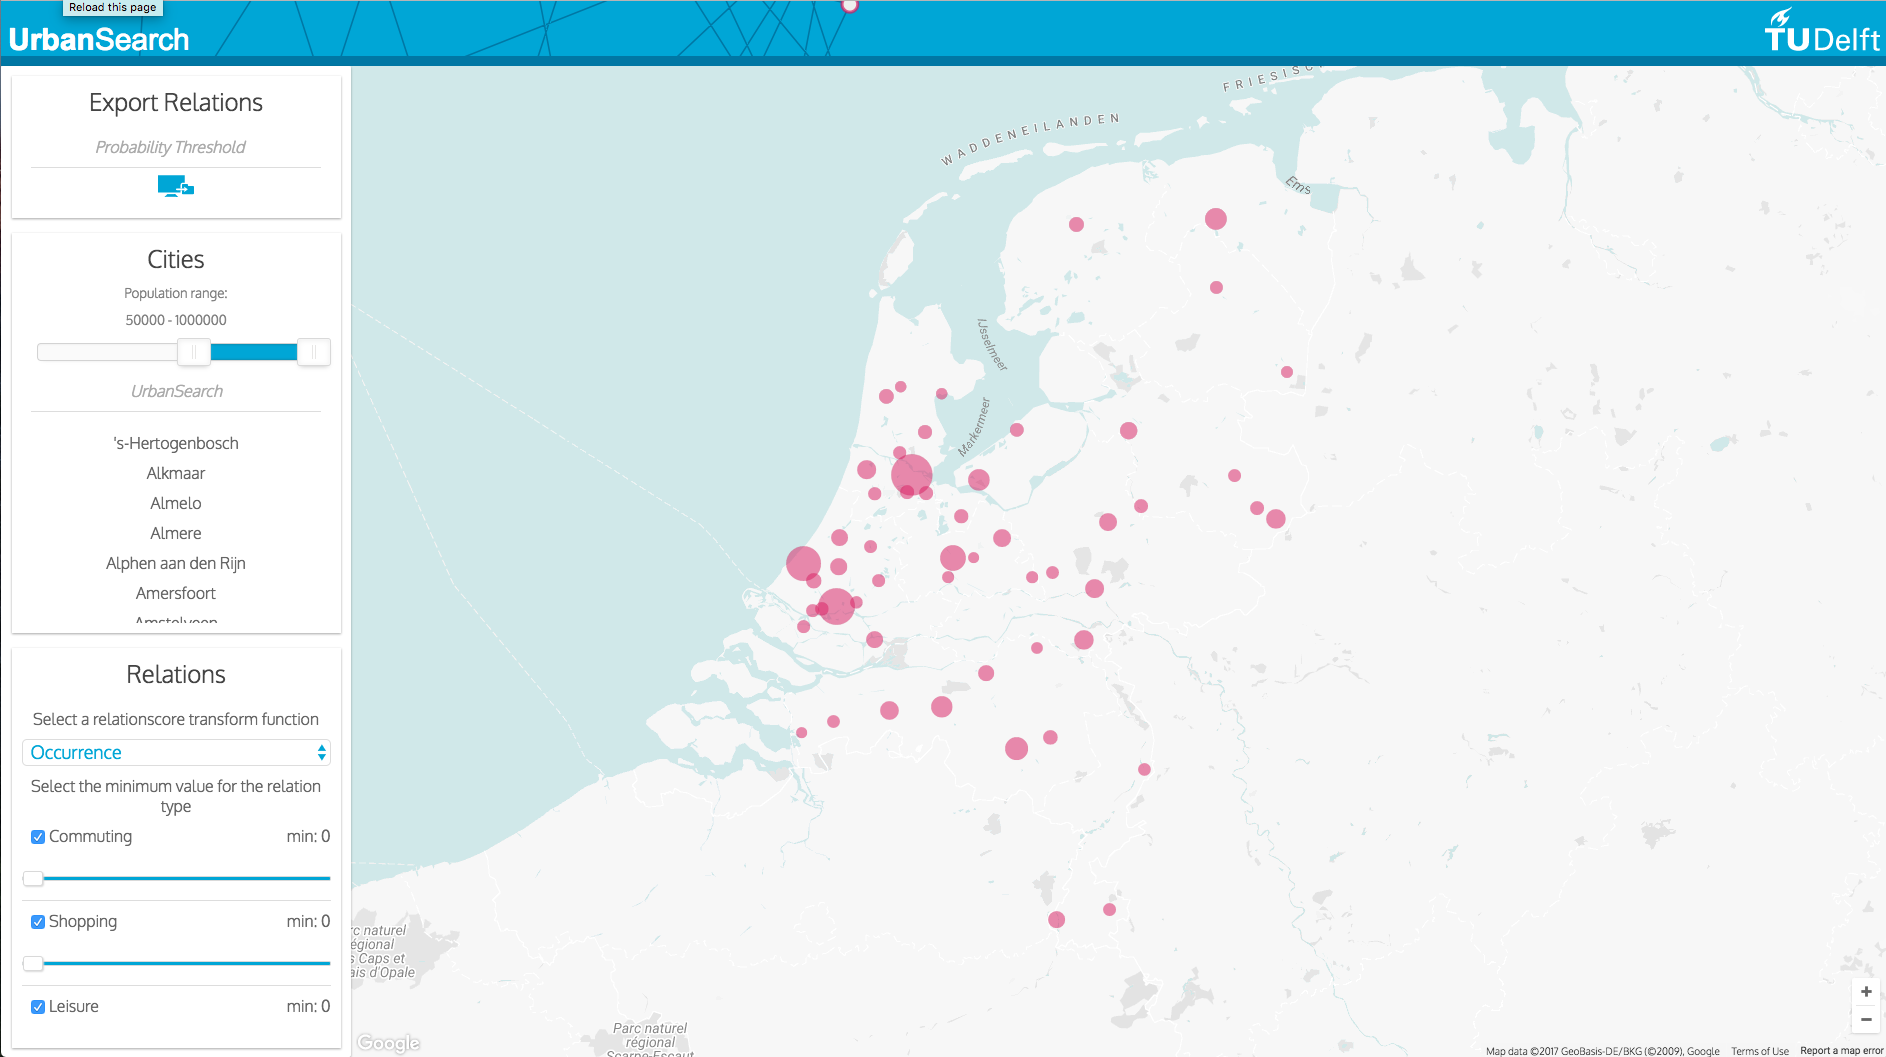
\includegraphics[width=.8\linewidth]{map.png}
    \caption{The interactive map with one relation selected}
    \label{fig:map}
\end{figure}

\subsection{Cities}\label{sec:city}
Cities are represented by circles which are drawn on the map and placed in the correct position using the latitude/longitude properties belonging to the city. We scale the circle based on the size of the population of the city. An example of a city on the map is show in figure \ref{fig:map-city}.

\begin{figure}[H]
  \centering
  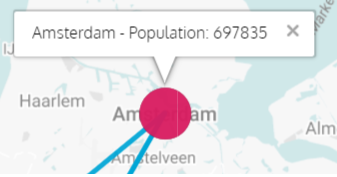
\includegraphics[width=.4\linewidth]{hover}
  \caption{Hovering over a city will display extra information about the city}
  \label{fig:map-city}
\end{figure}

When a user hovers over a city on the map, a pop up will appear with extra information about that city.\\
If a city is clicked the relations to other visible cities are shown. Clicking on a selected city toggles the visibility of the previously displayed relations. To make clear for the user  which cities are selected and which are not, we lower the opacity of selected cities.

\subsection{Relations}

Relations between cities are visualised using Google Maps Polylines\footnote{\url{https://developers.google.com/maps/documentation/javascript/3.exp/reference\#Polyline}}. Relations for a particular city are shown when a city node is selected as described in \ref{sec:city}.\\
\begin{figure}[H]
  \centering
  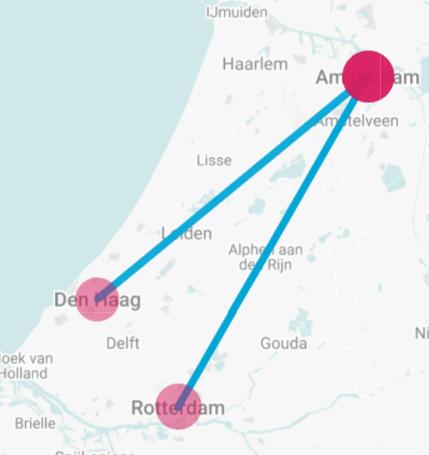
\includegraphics[width=.4\linewidth]{click}
  \caption{Selected city showing relations to other visible cities}
  \label{fig:sub2}
\end{figure}

Clicking on a relation opens up a new card containing information about this relation. The details about this card are discussed in \ref{sec:rel-info}.\\
The opacity of a relation indicates the relative strength of the relation compared to the relation with the highest score in the system. An example is given in figure \ref{fig:relation-opacity}.

\begin{figure}[H]
  \centering
  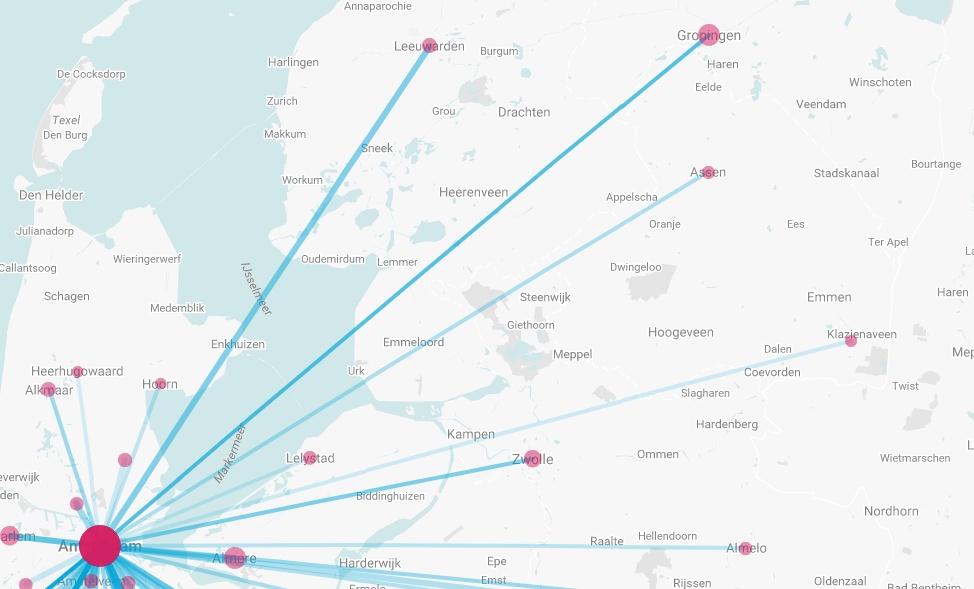
\includegraphics[width=.8\linewidth]{relation-opacity}
  \caption{A higher opacity indicates a weaker relative total strength of the relation. So Groningen has a stronger connection with Amsterdam then Assen.}
  \label{fig:relation-opacity}
\end{figure}


\subsection{Sidemenu}
The side-menu displayed in figure \ref{fig:sidemenu} allows the user to control the information that is displayed on the map. It is also the . The basic layout of the sidemenu is displayed in figure \ref{fig:sidemenu}. First we will discuss the elements that are always available in the sidemenu. Finally we will discuss dynamic content that can be added and removed from the sidemenu.

\begin{figure}[H]
    \centering
    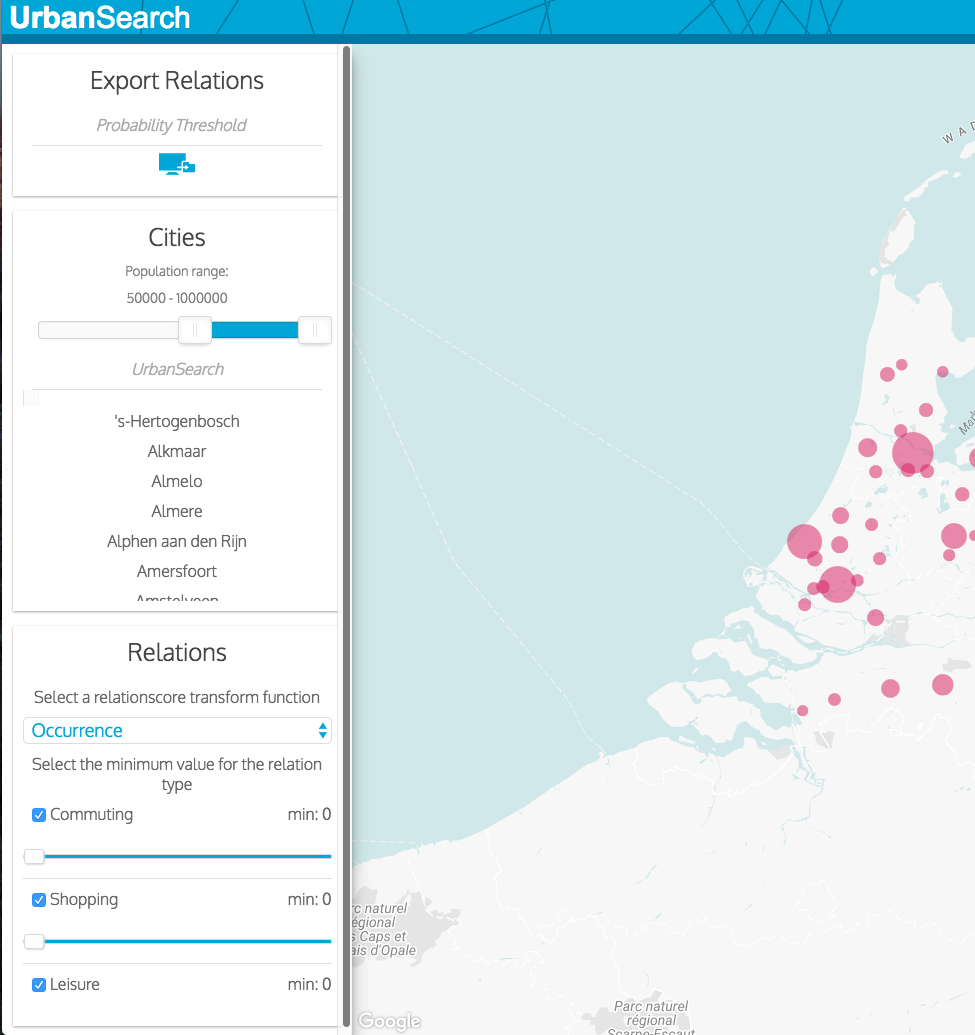
\includegraphics[width=.6\linewidth]{sidemenu}
    \caption{The sidemenu displayed on the left side of the interface}
    \label{fig:sidemenu}
\end{figure}


\subsubsection{City Controls}
The city controls displayed in figure \ref{fig:city-control} allow users to control the visibility of cities and city relations.\\
The population slider can be used to set the visibility of cities. All cities with a population size that is in the selected range are displayed on the map.\\
The search input allows the user to search a list of visible cities. When a city in the list is clicked, the relations for this city are shown on the map.

\begin{figure}[H]
    \centering
    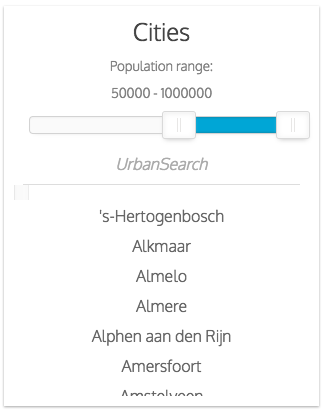
\includegraphics[width=.4\linewidth]{city-control}
    \caption{The city control card}
    \label{fig:city-control}
\end{figure}

\subsubsection{Relation Controls}
Using the relation controls displayed in figure \ref{fig:rel-control} an user can manipulate how intercity relations are displayed.\\
First of all the user can select several "transforms" from the drop-down that is available in the relation controls card. These transforms calculate a new value for the relation strengths based on the original values of the relations (which basically means the count of documents per category gets transformed for every relation). After the transform new totals and opacities are calculated for every relation. This way an user can quickly asses the difference of intercity relations for several relative measures.\\

\begin{figure}[H]
    \centering
    \begin{minipage}{0.9\textwidth}
        \centering
        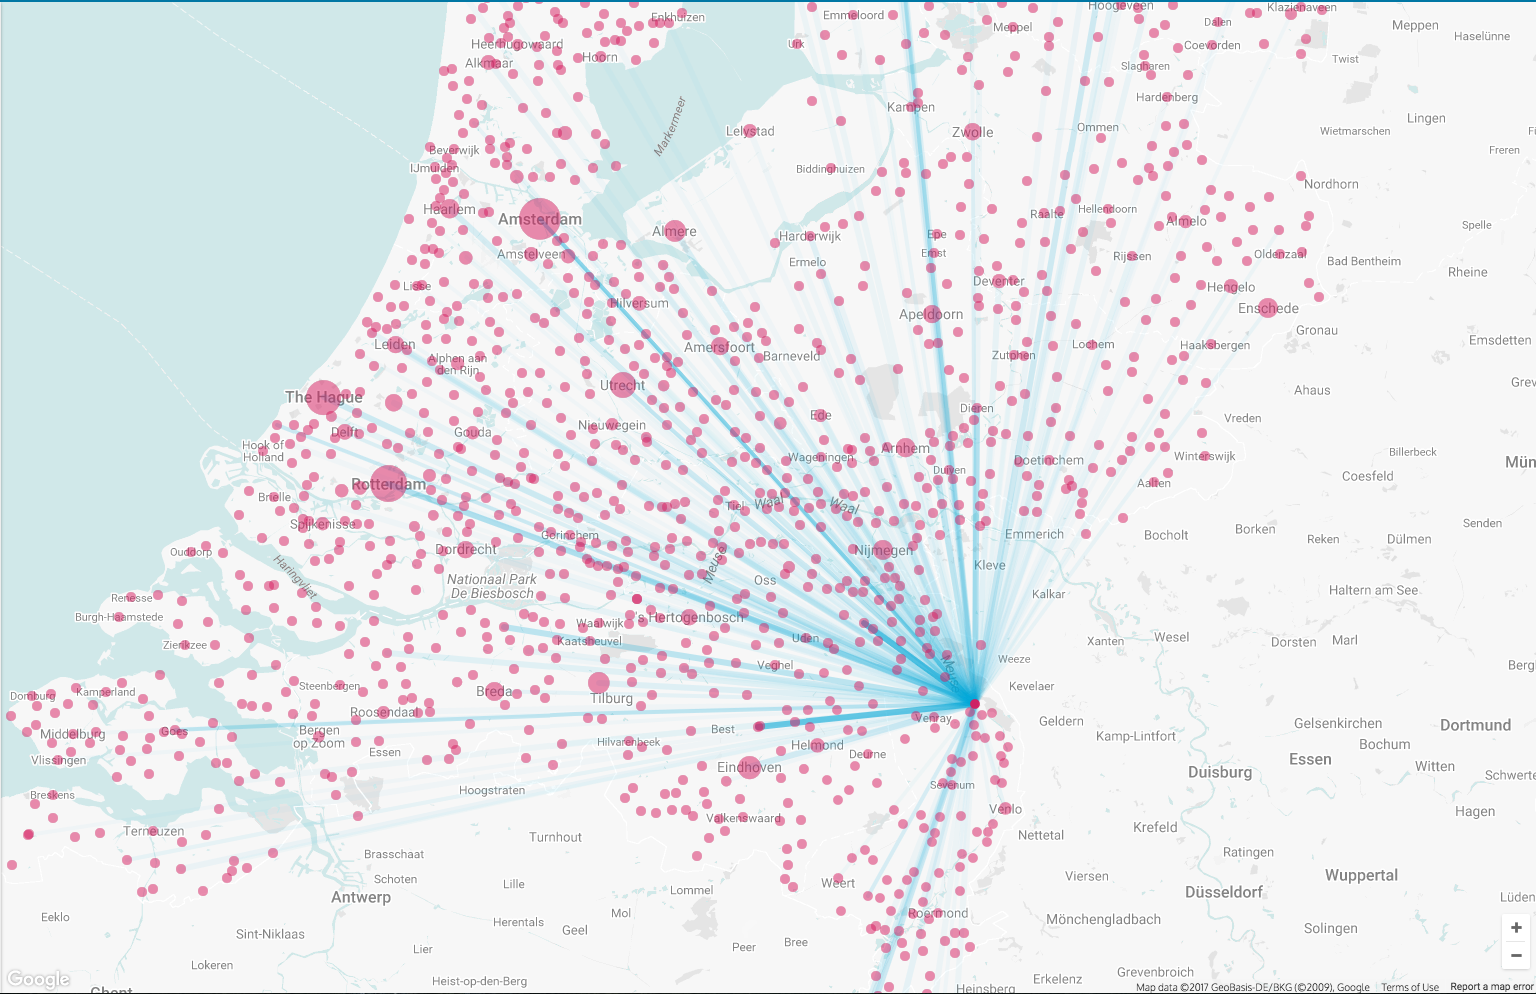
\includegraphics[width=0.9\textwidth]{rel-trans-occ}
        \caption{Opacity scaling based on total occurrences}
        \label{fig:rel-trans-occ}
    \end{minipage}\hfill
    \begin{minipage}{0.9\textwidth}
        \centering
        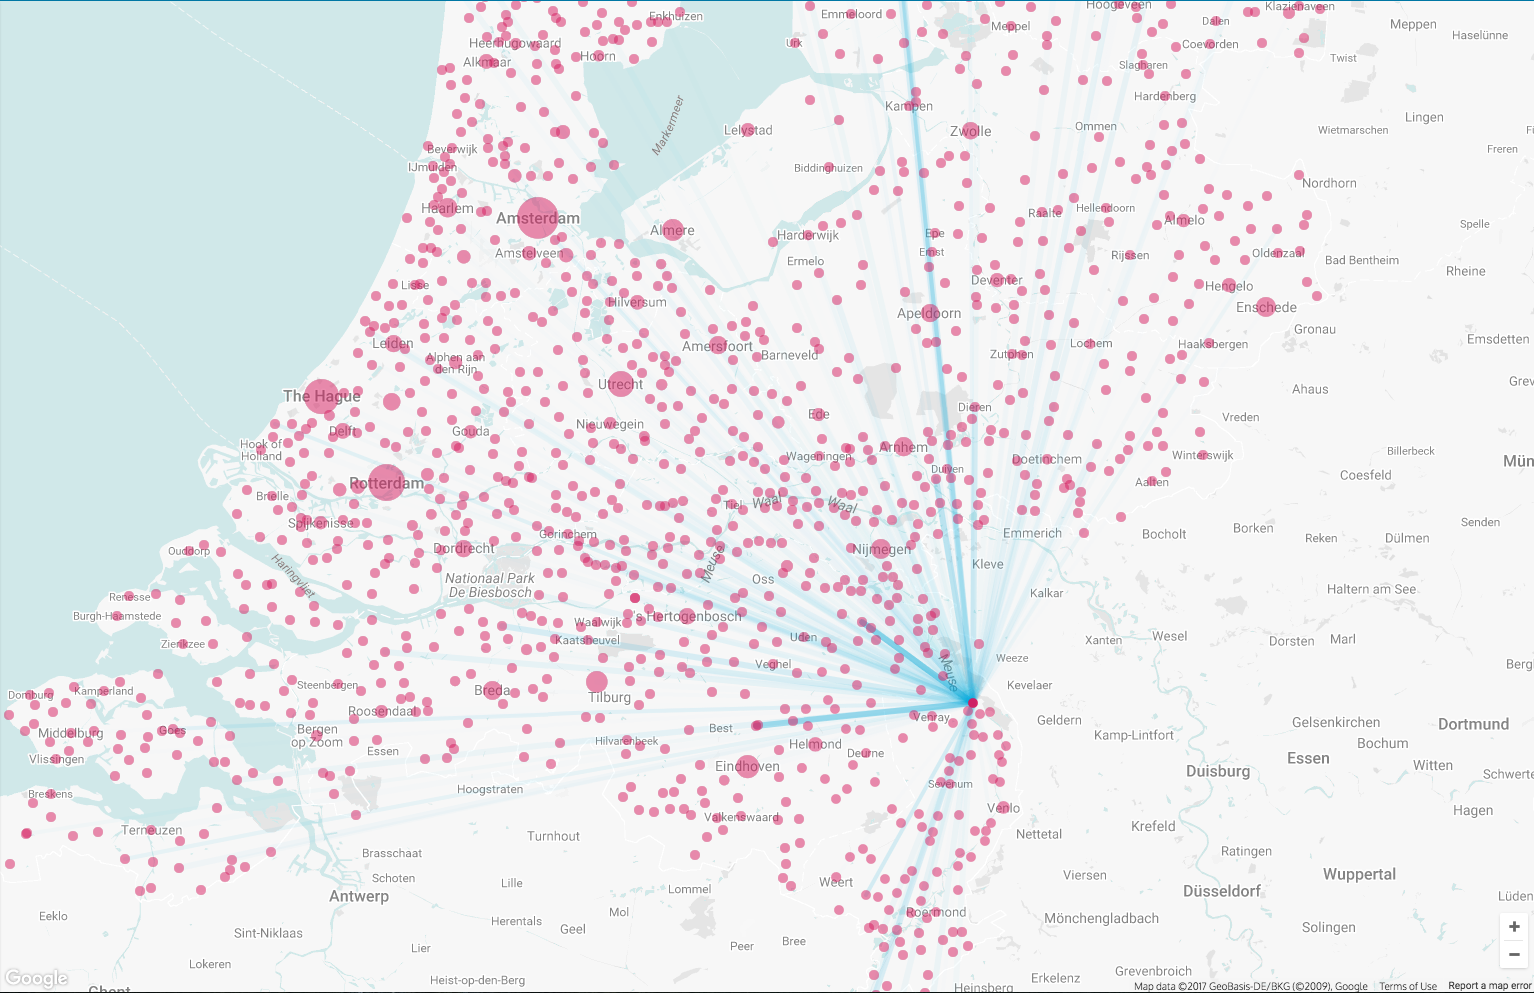
\includegraphics[width=0.9\textwidth]{rel-trans-pop}
        \caption{Opacity scaling based on total occurrences over minimum population size of a relation}
        \label{fig:rel-trans-pop}
    \end{minipage}
    \label{fig:rel-trans}
\end{figure}
% \begin{figure}[H]
%     \centering
%     \begin{subfigure}
%         \centering
%         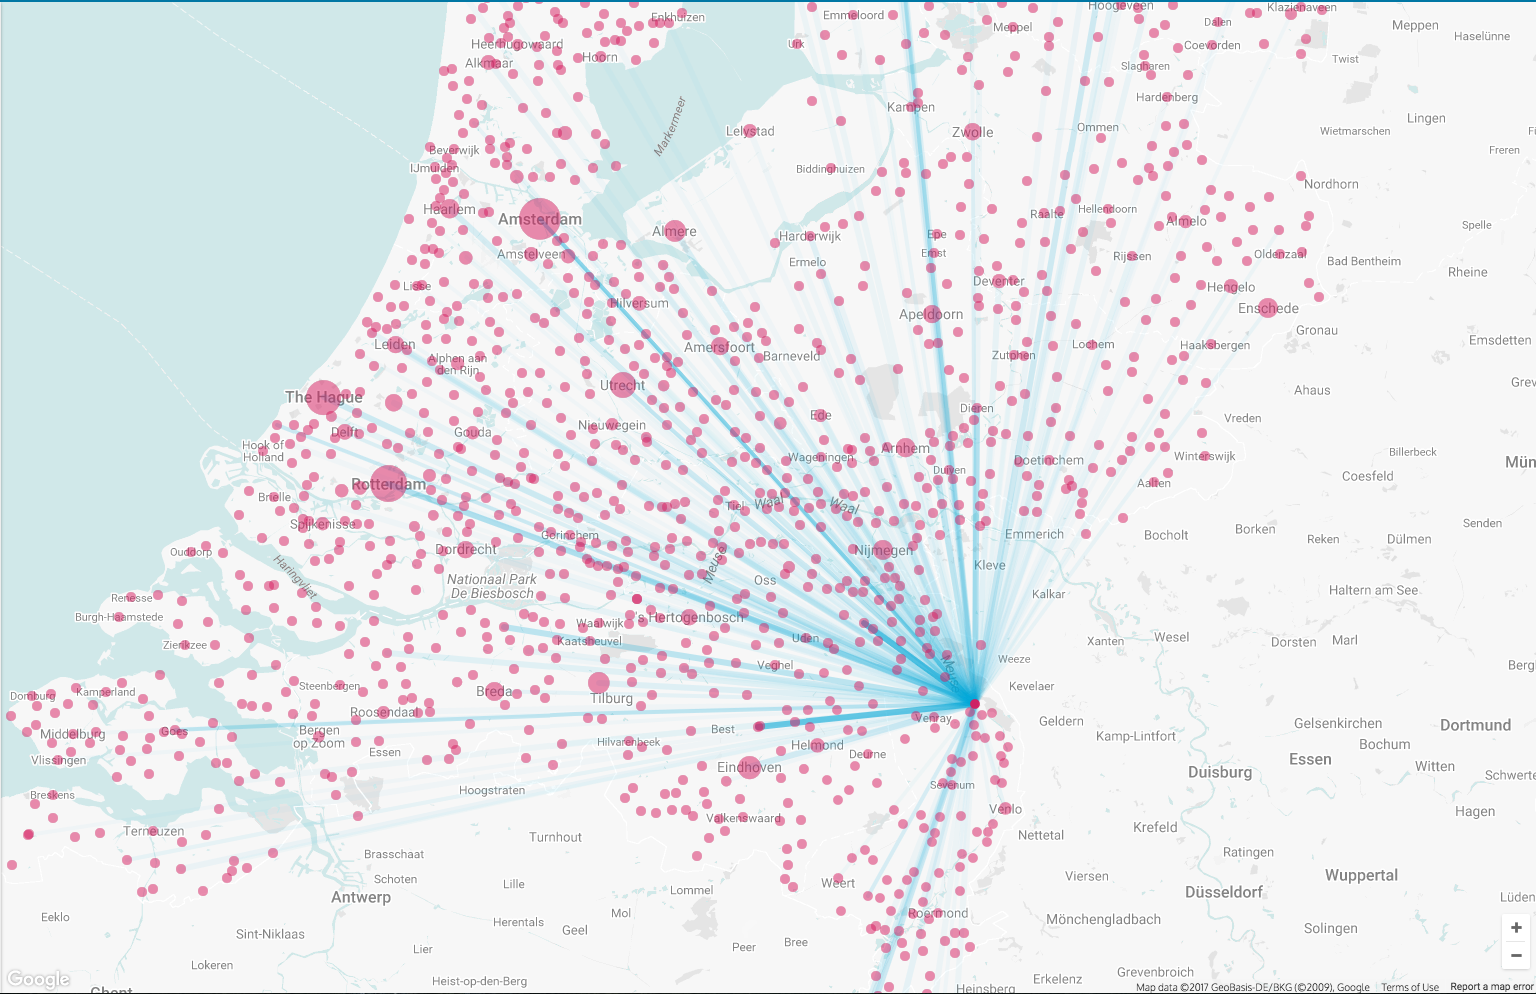
\includegraphics[width=.4\linewidth]{rel-trans-occ}
%         \caption{Opacity scaling based on total occurrences}
%         \label{fig:rel-trans-occ}
%     \end{subfigure}
%     \begin{subfigure}
%         \centering
%         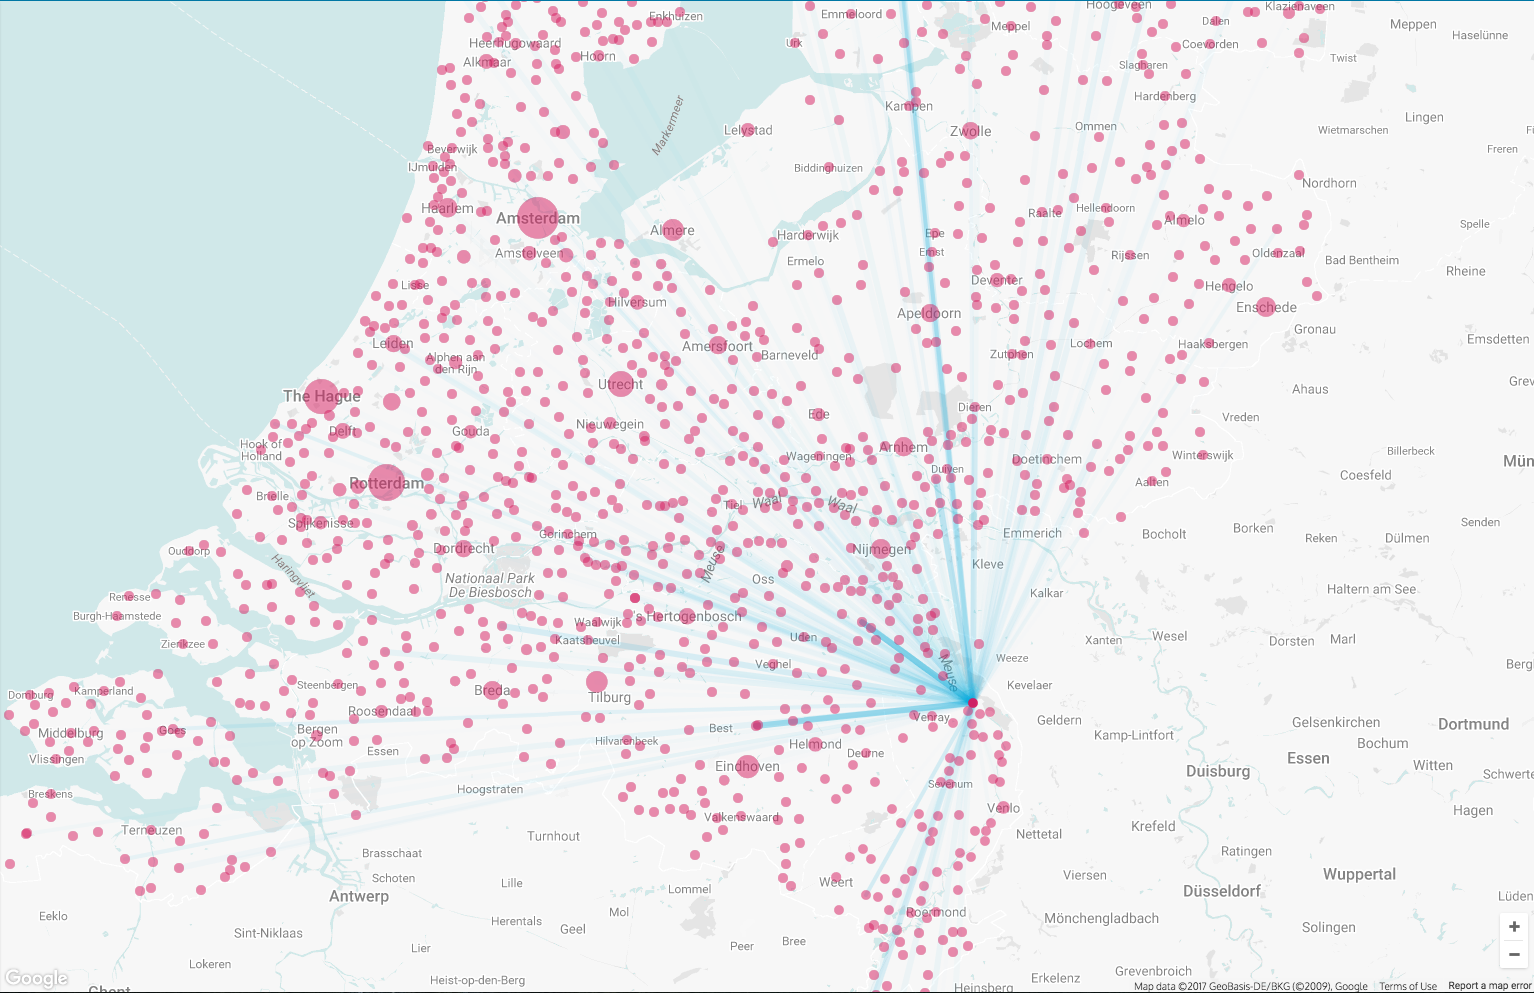
\includegraphics[width=.4\linewidth]{rel-trans-pop}
%         \caption{Opacity scaling based on total occurrences over minimum population size of a relation}
%         \label{fig:rel-trans-pop}
%     \end{subfigure}
%     \label{fig:rel-trans}
% \end{figure}

Using the sliders for each category a user can set a minimum threshold for a relation category strength. For example if the value for the category "education" is set to 25 all relations that have a score lower than 25 on "education" are hidden.
Finally relation categories can be selected and deselected. This triggers an update of the total relation strengths, respectively adding to or subtracting from the total relation score the score of the toggled category.


\subsubsection{Export}
In the export card an user can download all the relations in the system in CSV format. If the user provides an threshold \todo{PIET ZEG FF WAT ER PRECIES GEBEURT}.

\begin{figure}[H]
    \centering
    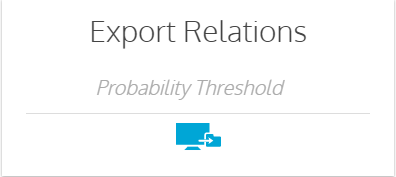
\includegraphics{export}
    \caption{the export card}
    \label{fig:infoflow}
\end{figure}

\subsubsection{Relation Information}\label{sec:rel-info}

When clicking on a relation an extra window in the menu will be opened. This contains all information about the relation between the two cities. The strength of the relations (amount of documents found for the relation between those cities) will be displayed, as well as the strength of the relations per category (such as commuting, shopping, leisure, etc.).\\
To provide the user with the option to validate the results, a "Get Documents" button, at the bottom of this card, fetches all the documents that belong to this relation.


\begin{figure}[H]
    \centering
    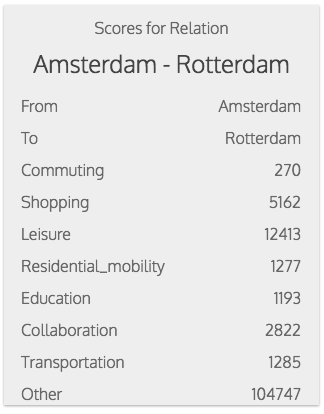
\includegraphics[width=0.4\textwidth]{rel-scores}
    \caption{Relations scores between two cities}
    \label{fig:rel-scores}
\end{figure}

\subsubsection{Relation Documents}\label{sec:rel-docs}

In this card all documents, that are assigned to the selected relation, will be displayed. The documents are listed as shown figure \ref{fig:classification}. Each listed item shows the category with which it has been labelled using our classifier. It also shows the probability with which this document was assigned to this category.\\
If a user wants to inspect the contents of a certain file a list item can be clicked, which will initiate the download of the selected document.

\begin{figure}[H]
    \centering
    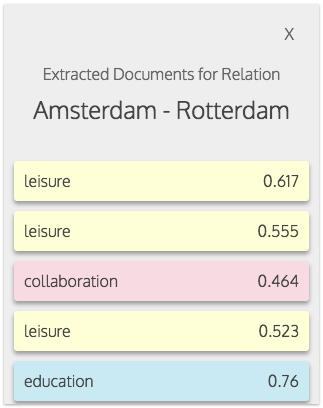
\includegraphics[width=0.4\textwidth]{rel-docs}
    \caption{Documents included in relations}
    \label{fig:rel-docs}
\end{figure}


\section{Classification Interface}

The classification interface is meant as an easy to use tool for extending the systems training-set. From our document set, which we have filtered from all the CommonCrawl pages, we fetch a random document. This document is displayed in the interface shown in figure \ref{fig:classification}. The user can select one or more categories to tag this document, after which the user can hit the submit button to save the document to our training set.\\
If a user deems the document to be of no use for any of the categories, the document can be discarded by clicking the "discard" button.\\
Finally if the user wants to add his or her own documents this can be done by hitting the "clear" button and copy-pasting the contents of the documents into the document field, selecting one or more matching categories and submitting the document.

\begin{figure}[H]
    \centering
    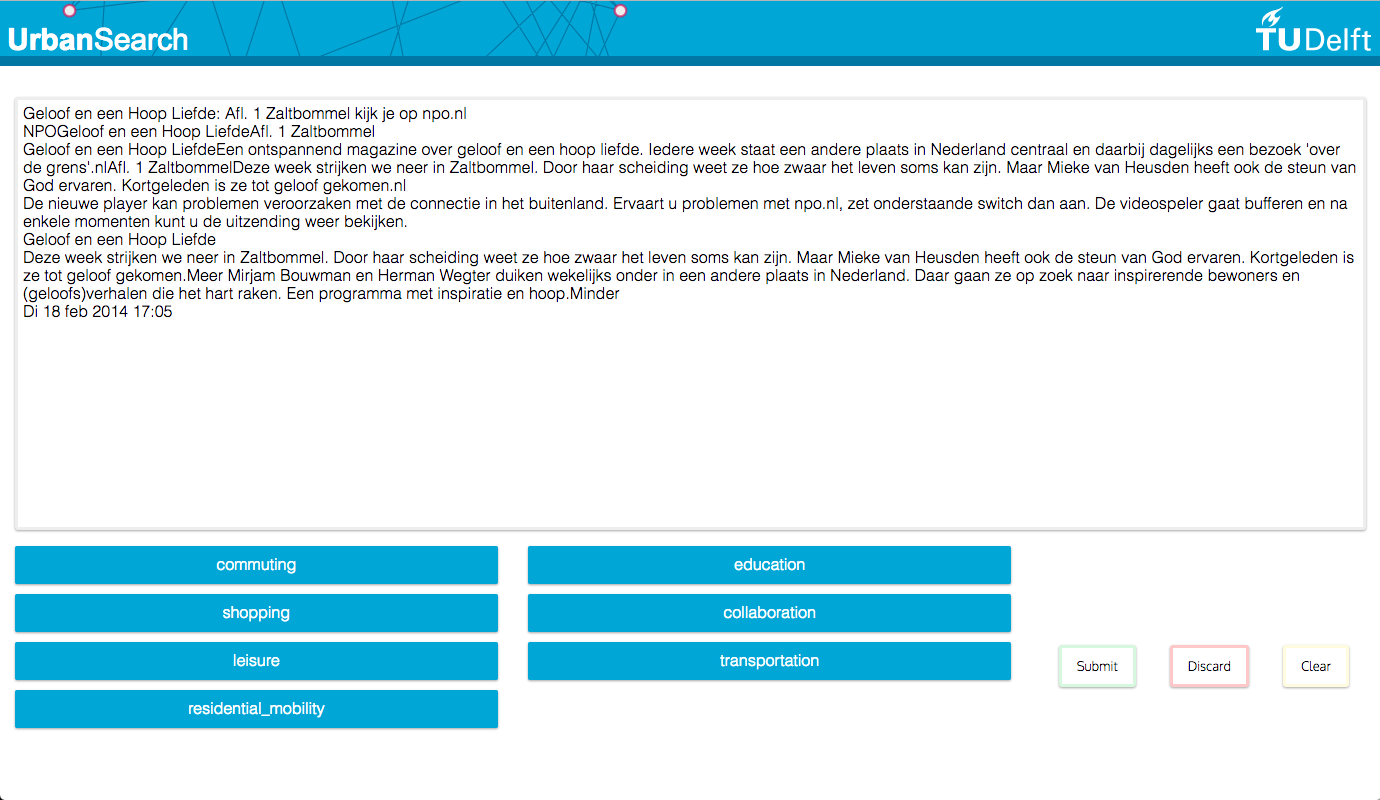
\includegraphics[width=1\textwidth]{classification}
    \caption{The classification interface}
    \label{fig:classification}
\end{figure}

\section{Classifier Interface}

Finally we have the classifier interface. This interface provides us with a way to train a new default classifier which is used by the system for the API and for classification.\\
A new classifier can be trained by clicking the "Train!" button. If all goes well, the "Train!" button will change to a "Done!" button, indicating the successful creation of a new default classifier for the system.\\ 
Although we can train a new default classifier, this classifier will not be used by the system until the complete system is restarted.\\
The bottom part of the classifier page consists of tiles providing the user with information about the size of the training set.

\begin{figure}[H]
    \centering
    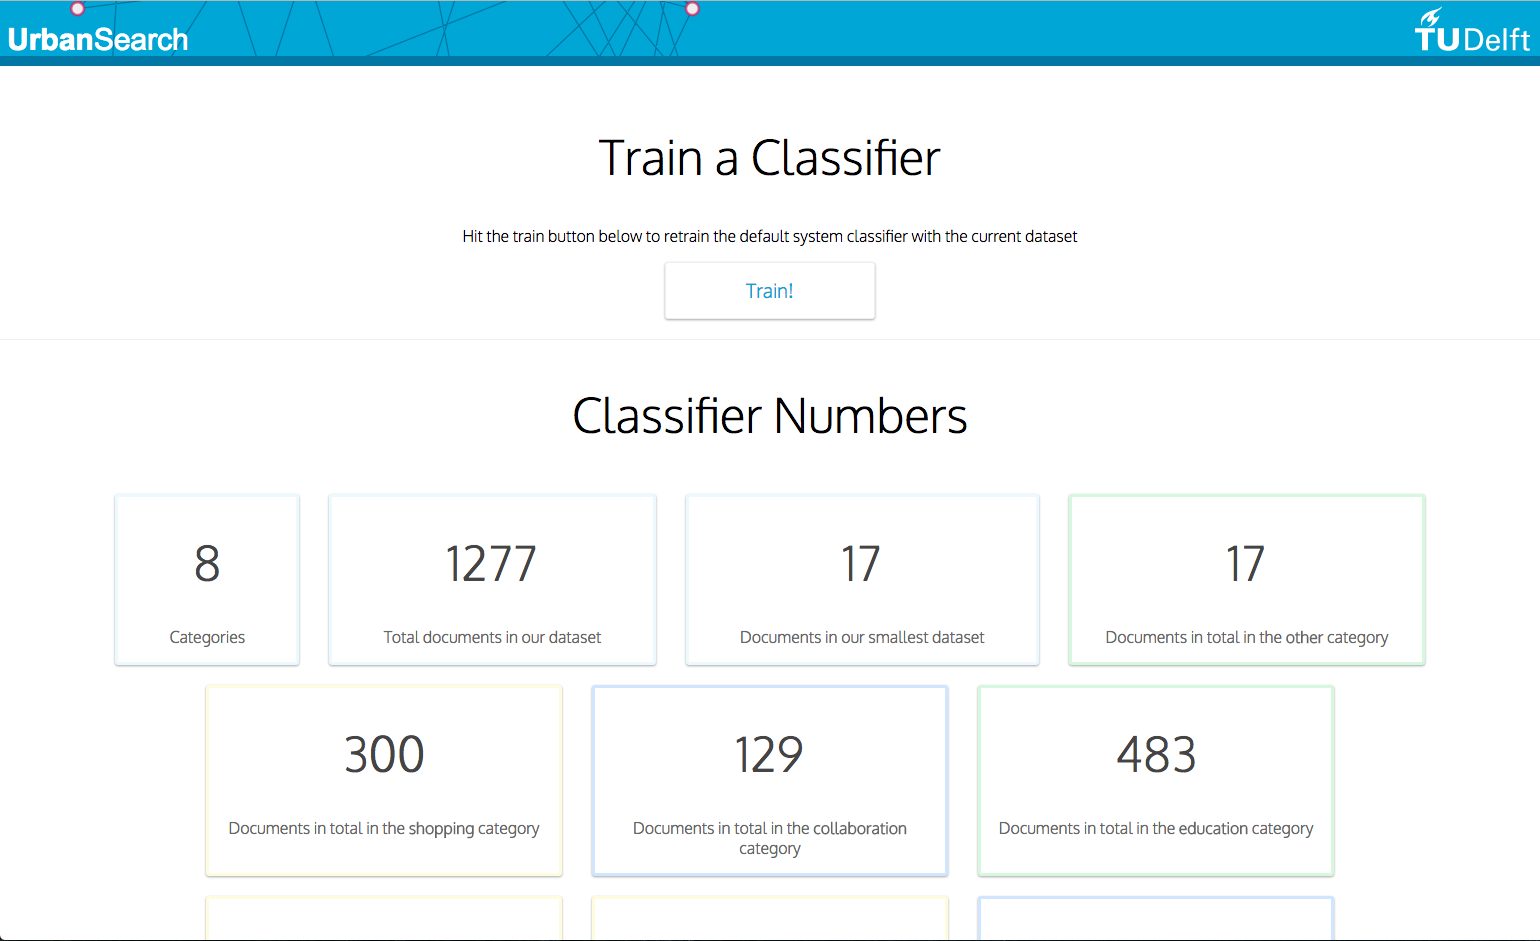
\includegraphics[width=1\textwidth]{classifier}
    \caption{The classifier interface}
    \label{fig:classifier}
\end{figure}
